\section{Method}

%%% Definition: CutMix %%%
Recall that CutMix pastes a box of one image onto another and mixes the two labels in
proportion to the area that each image keeps.
%%% end %%%

%%% Method: Training setup %%%
We train a ResNet-50 for 200 epochs with SGD, a cosine schedule and a batch size of 256. CutMix is
applied to every batch with $\lambda \sim \mathrm{Beta}(1, 1)$.
%%% end %%%
All numbers are averaged over 5 seeds.

%%% Figure: Training loss %%%
\begin{figure}[t]
  \centering
  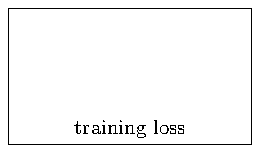
\includegraphics[width=.8\linewidth]{figures/loss.pdf}
  \caption{Training loss}\label{fig:training-loss}
\end{figure}
%%% end %%%

%%% Lemma: Mixing bound %%%
\begin{lemma}[Mixing bound]\label{lem:mixing-bound}
The mixed label $\tilde{y}$ lies in the convex hull of $y_A$ and $y_B$.
\end{lemma}
%%% end %%%
